%
% File emnlp2015.tex
%
% Contact: daniele.pighin@gmail.com
%%
%% Based on the style files for ACL-2015, which were, in turn,
%% Based on the style files for ACL-2014, which were, in turn,
%% Based on the style files for ACL-2013, which were, in turn,
%% Based on the style files for ACL-2012, which were, in turn,
%% based on the style files for ACL-2011, which were, in turn, 
%% based on the style files for ACL-2010, which were, in turn, 
%% based on the style files for ACL-IJCNLP-2009, which were, in turn,
%% based on the style files for EACL-2009 and IJCNLP-2008...

%% Based on the style files for EACL 2006 by 
%%e.agirre@ehu.es or Sergi.Balari@uab.es
%% and that of ACL 08 by Joakim Nivre and Noah Smith

\documentclass[11pt,a4paper]{article}
\renewcommand{\baselinestretch}{1.035}
\usepackage{acl2015}
\usepackage{times}
\usepackage{url}
\usepackage{latexsym}
\usepackage{amsmath}
\usepackage{color}
\usepackage{epsfig,url,algorithm,algorithmic,multirow}
\usepackage{amssymb}

\newtheorem{theorem}{Theorem}
\newtheorem{lemma}{Lemma}
\newtheorem{corollary}{Corollary}
\newtheorem{definition}{Definition}
\newtheorem{example}{Example}
\newtheorem{hypothesis}{Hypothesis}

%\setlength\titlebox{5cm}

% You can expand the titlebox if you need extra space
% to show all the authors. Please do not make the titlebox
% smaller than 5cm (the original size); we will check this
% in the camera-ready version and ask you to change it back.


\title{``A Spousal Relation Begins with a Deletion of \textit{engage} \\and Ends with an Addition of \textit{divorce}": \\
Learning State Changing Verbs from Wikipedia Edit History}
%Ndapa: title is too long, so leavig this out
%\\Mapping Text and Infobox Changes in Wikipedia to \\Learn Verbs and State Changes for Knowledge Base Updates}

\author{%Derry Tanti Wijaya \\
  %Carnegie Mellon University \\
  %5000 Forbes Avenue \\
  %Pittsburgh, PA, 15213 \\
  %{\tt dwijaya@cs.cmu.edu} \\\And
   %Ndapandula Nakashole \\
  %Carnegie Mellon University \\
  %5000 Forbes Avenue \\
  %Pittsburgh, PA, 15213 \\
  %{\tt ndapa@cs.cmu.edu} \\\And
  %Tom M. Mitchell \\
  %Carnegie Mellon University \\
  %5000 Forbes Avenue \\
  %Pittsburgh, PA, 15213 \\
  %{\tt tom.mitchell@cs.cmu.edu} \\
  }

\date{}

\begin{document}

\maketitle

%\vspace{-1cm} %ineffective here anyway

\begin{abstract}
%Ndapa: this abstact intro is a bit stale and over used as we have used it in 
% the other papers, I have changed it a bit and also made the abstract shorter.
% it is better to keep the abstract short and give more motivation in the intro

%Knowledge bases (KBs) %that have emerged 
%that have emerged in recent years  are mostly static. They contain facts about the world yet are seldom updated. This paper proposes a %method for learning state changes brought about by verbs acting on their arguments (i.e., entities).
% State changes are viewed as updates of KB facts pertaining to the entities. 

Learning to determine when the facts of a Knowledge Base (KB) have to be updated is a challenging task.
We propose to learn state changing verbs from Wikipedia edit history. When a state-changing event,  such as a marriage or death,  happens to an entity, the  infobox on the entity's Wikipedia page usually gets  updated. At the same time, the  article text may be updated with verbs either being added or deleted to reflect the changes made to the infobox. We use Wikipedia edit history %histories 
to distantly supervise a method for automatically learning verbs and state changes. Additionally, our method uses %fact-specific 
constraints
 %such as mutually exclusivisity vs. simultaneous changes of infobox slots
  to effectively map verbs to infobox changes. We observe in our experiments that when state-changing verbs are  added or deleted from an entity's Wikipedia  page text, we can update the entity's infobox updates with 88\% precision and 76\% recall.
One compelling  application of our verbs is to incorporate them as triggers in methods for   updating existing KBs, which are currently mostly static.

\end{abstract}
\section{Introduction}

\begin{figure*}[t]
\begin{center}
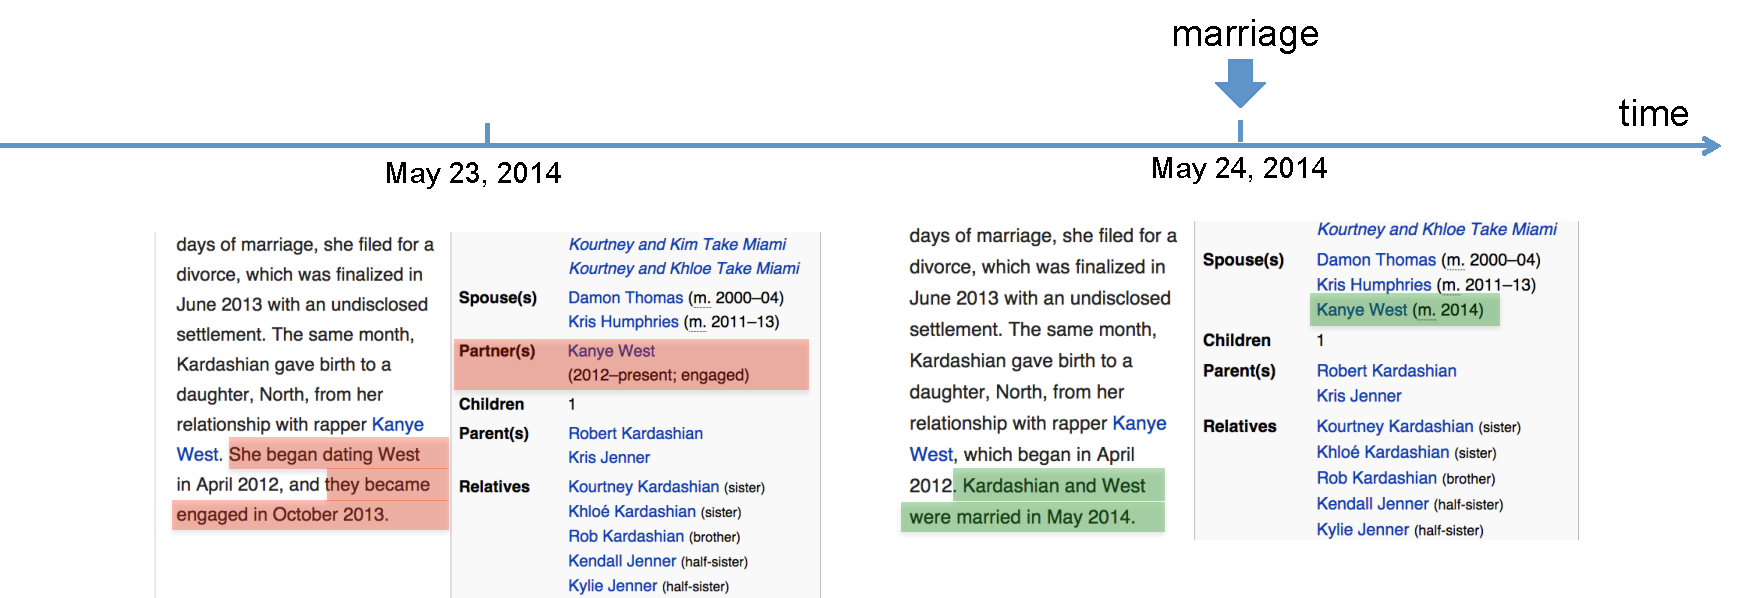
\includegraphics[width=14cm,keepaspectratio=true]{figures/motivation.pdf}
\caption{\label{fig:motivation} A snapshot of Kim Kardashian's Wikipedia revision history, highlighting text and infobox changes. In red (and green) are the difference between the page on May 23 and May 24, 2014: things that are deleted from (and resp. added to) the page.}
\end{center}
\end{figure*}

In recent years there has been a lot of research on extracting relational facts between entities and storing them in knowledge bases (KBs). These knowledge bases such as YAGO (which extract facts from Wikipedia infoboxes \cite{suchanek2007yago}) or NELL (which extracts facts from any Web text \cite{carlson2010toward,fader2011identifying}) are generally static. They are not updated as the Web changes when in reality new facts arise while others cease to be valid%or change over time
. One approach towards real-time population of KBs is to extract facts from dynamic content of the web such as news \cite{nakashole2012real}. This paper proposes a \textit{shift} of focus from doing KB updates by extracting facts in text to doing them by identifying state changes brought about by verbs in text. 

The benefit of such shift is multi-fold: (1) Detecting state change to an entity in text can be used to infer and update the entity's fact and its temporal scope in KB \cite{wijayactp}. (2) Learning state changes brought about by verbs can pave ways to learning the pre- and post-conditions of state-changing verbs: the entry condition (in terms of KB facts) that must be true for an event expressed by the verb to take place, and the exit condition (in terms of KB facts) that will be true after the event occurs. Such pre- and post-conditions can be useful for (a) learning event sequences %such as scripts \cite{schank2013scripts}, which can be modeled
as a collection of verbs chained together by pre- and post-condition of their shared entities, (b) for inferring cascading effect of an event via the pre- and post-condition of shared entities in an event sequence, or (c) for inferring unknown states of entities from the verbs they participate in.  

In this paper, we propose to learn state changes brought about by verbs using Wikipedia revision histories. Our assumption is that when a state-changing event happens to an entity e.g., a marriage, its Wikipedia infobox: a structured document that contains a set of facts (attribute-value pairs) of the entity is updated e.g., by the addition of a new \textsc{spouse} value. At the same time, texts that contain verbs that express the event e.g., \textit{wed} may be added to the entity's Wikipedia page (see an example in Figure \ref{fig:motivation}). Wikipedia revisions over many entities can act as distantly supervised data for mapping text and infobox changes that relate to events. However, Wikipedia revisions are \textit{noisy}: there is no guarantee that only the infobox slots related to a particular event will be updated. For example, when an event such as death happens, slots regarding birth e.g., \textit{birthdate}, \textit{birthplace}, may also be updated. To alleviate the effect of such, we leverage constraints between slots e.g., that \textit{deathdate} is mutually exclusive with \textit{birthdate} or that \textit{birthdate} is simultaneously updated with \textit{birthplace}, to effectively learn infobox changes that relate to a particular event-expressing verb. 

Our contribution is the construction and use of an interesting, distantly labeled, dataset from Wikipedia revisions for learning about verb and state changes\footnote[1]{We make our dataset available here: http://.../wiki-edits-dataset.zip}, and the learned resource of verbs effective for identifying state changes.
\section{Method} \label{sec:method}

\subsection{Data Construction}
We construct a dataset from Wikipedia revision histories of person entities whose facts change between the year 2007 and 2012 (i.e., have at least one fact in YAGO KB with a start or end time in this period). We obtain Wikipedia URLs of this set of entities $P$ from YAGO and crawl their revision histories%, obtaining any revision their pages have between the year 2007 and 2012
. Given a person $p$, his Wikipedia revision history $H_p$ has a set of ordered dates $T_p$ on which revisions are made to his Wikipedia page $W_p$ (we consider a date granularity for time). Each revision $W_{p, t_p} \in H_p$ is the content of $W_p$ at date $t_p$ where $t_p \in T_p$. 

A document $d_{p, t_p}$ in our data set is the \textit{difference}\footnote[2]{a HTML document obtained by ``compare selected revisions"  functionality in Wikipedia} between any two consecutive revisions to $W_p$ that is separated by at least a single date worth of revisions i.e., $d_{p, t_p} = W_{p, \overline{t_p+2}} - W_{p, \underline{t_p}}$. Where $W_{p, \overline{t_p+2}}$ is the \textit{first} revision on date $t_p+2$ and $W_{p, \underline{t_p}}$ is the \textit{last} revision on date $t_p$ (since $W_p$ can be revised multiple times on a date). Our dataset consists of all documents $d_{p, t_p}$, $\forall t_p \in T_p,\ t \in [01/01/2007,\ 12/31/2012]$, and $\forall p \in P$; a total of 288,184 documents from revision histories of 16,909 Wikipedia entities.

%For example, Ralph McInerny's Wikipedia page was consecutively revised on the dates of 11/20/2012, 12/26/2012 and 12/29/2012. We find the difference between the last revision to his page on 11/20/2012 and the first revision to his page on 12/29/2012 (since a page can be revised multiple times in a date). This difference\footnote[2]{http://en.wikipedia.org/w/index.php?title=Ralph\_McInerny \&type=revision\&diff=530257160\&oldid=523980632}, a HTML page obtained by ``compare selected revisions"  functionality in Wikipedia, is a document in our dataset. Using this method, we obtain 288,184 documents from revision histories of 16,909 Wikipedia entities. 

Each Wikipedia revision $W_{p, t_p}$ consists of a set of infobox slots $S$ and a textual content $C$, where each slot $s \in S$ is a quadruple, $\langle s_{att}$, $s_{value}$,  $s_{start}$, $s_{end} \rangle$ containing the attribute name (non-empty), the attribute value, and the start and end time for which this attribute-value pair is valid. 

Each document in our datase is a \textit{difference} between $W_{p, t_p+2} - W_{p, t_p}$, and therefore consists of a set of infobox changes $\Delta S$ and textual changes $\Delta C$. Each slot change $\delta s \in \Delta S$ is also a quadruple %$\langle s_{att}$, $s_{value}$,  $s_{start}$, $s_{end} \rangle$ 
but where $s_{value}$,  $s_{start}$, or $s_{end}$, whenever not empty, is prefixed with $+$ or $-$ to indicate whether they are being added to or deleted in the newer revision $W_{p, t_p+2}$. Similarly, each content change $\delta c \in \Delta C$ is prefixed with $+$ or $-$ indicating whether they are an addition or deletion in $W_{p, t_p+2}$. %For the content, we focus on verbs by extracting (lemmatized) verb phrases from the content change which has subject matched $p$ and object matched $\delta s$ value $s_{value}$ or vice versa.
For example, in Figure \ref{fig:motivation}, a document constructed from the difference $W_{kim, 05/25/2014} - W_{kim, 05/23/2014}$ consists of slot changes: $\langle\textsc{spouse}$, \textbf{$+$}``Kanye West",  $+$``2014", `` "$\rangle$, $\langle\textsc{partner}$, $-$``Kanye West",  $-$``2012-present; engaged", `` "$\rangle$ and content changes: $+$``Kardashian and West were married in May 2014", $-$``She began dating West", $-$``they became engaged in October 2013".

We label documents that have $\langle s_{att}, +s_{value}, *, *\rangle$ or $\langle s_{att}, *, +s_{start}, *\rangle$ $\in \Delta S$ with the label \textit{begin-}$s_{att}$ and documents that have $\langle s_{att}, *, *, +s_{end}\rangle$ $\in \Delta S$ with the label \textit{end-}$s_{att}$. The label represents the state change that happens in the document. Since a document can have more than one slot changes, it can have more than one labels. %if it has more than one $\delta s$ with qualifying value, start or end time. 
For example, in Figure \ref{fig:motivation}, a document constructed from the difference $W_{kim,\tiny 05/25/2014\normalsize } - W_{kim, \tiny 05/23/2014\normalsize }$ is labeled with \textit{begin-spouse} and \textit{end-partner}. 

We use 90\% of our labeled documents as training and test on the remaining 10\%. We focus only on verbs that predict state change, hence for each labeled document we use as features only lemmatized verbs (verb or verb + preposition) in $\delta c$ whose subject matched the person $p$ and whose object matched any slot change value $s_{value}$ in the document (or vice versa). The task is then to predict for a document, the label of the document given its verbs features. 

%We define an infobox attribute of an entity e.g., \textsc{spouse} to \textit{begin} when a new value or a begin time is added to the attribute slot and to \textit{end} when an end time is being added to the slot. Using regular expression to detect whether a new value, a start, or an end time is being added to infobox slots of a document, we automatically label each document with ``begin-\{attribute\_name\}" or ``end-\{attribute\_name\}". So a document that contains an addition of a new value in the \textsc{spouse} slot will be labeled ``begin-spouse", while a document that contains an addition of end time in the \textsc{spouse} slot will be labeled ``end-spouse". 

\subsection{Model}


\section{Experiments}

\begin{figure}
\begin{center}
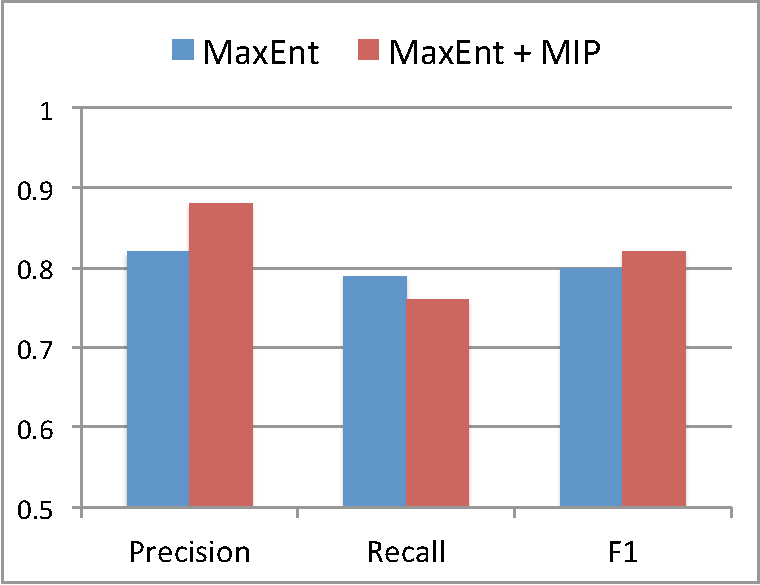
\includegraphics[width=8cm,keepaspectratio=true]{figures/result.pdf}
\caption{\label{fig:result} Results of predicting state change labels (infobox types) using verb features.}
\end{center}
\end{figure}

We use 90\% of our labeled documents that have verb edits as features (section \ref{sec:data}) as training data and test on the remaining 10\%. Since revision history data is noisy, we manually go through our test data to discard documents that have incorrect infobox  labels by looking the  text that  changed. The task is to predict for each document (revision), the label (infobox slot change) of the document given its verbs features. We compute precision, recall, and F1 values of our predictions  and compare the values before and after feature selection (Fig. \ref{fig:result}).

%\begin{table}
%\begin{small}
%\begin{center}
%\begin{tabular}{|l|r|r|r|}
%\hline
%Method & Precision & Recall & F1 \\
%\hline
%\textsc{MaxEnt} & 0.82 & 0.79 & 0.80 \\
%\hline
%\textsc{MaxEnt} + MIP & 0.88 & 0.76 & 0.82 \\
%\hline
%\end{tabular}
%\caption{\label{table:performance} Results of predicting state change label using verb features.}
%\end{center}
%\end{small}
%\end{table}

To the best of our knowledge, the task to learn state-changing verbs in terms of states defined in existing knowledge bases and learning it from Wikipedia edit histories is novel. There is no previous approach that can be used as baseline; therefore we have compared our structured prediction using MIP and \textsc{MaxEnt} with a majority class baseline. Both our approaches (\textsc{MaxEnt} and \textsc{MaxEnt} + MIP) perform better than the majority class baseline (Figure \ref{fig:result}). 

We observe the value of doing feature selection by asserting constraints in an MIP formulation. Feature selection improves precision; resulting in a better F1. By asserting constraints, some of the  inconsistent verb features for the labels were removed. For example, before feature selection, the verbs: ``marry", and ``be married to" were high-weighted features for both \textit{begin-spouse} and \textit{end-spouse}. After asserting constraints that \textit{begin-spouse} is mutex with \textit{end-spouse}, these verbs (whose base form is ``marry") are filtered out from the features of \textit{end-spouse}. We show some of the learned verb features (after feature selection) for some of the labels in (Table \ref{table:verbs}). In average, we have about 18 verbs per infobox state change in our state changing verb resource that we make available for future research. 



\begin{table}[t]
\begin{scriptsize}
\begin{center}
\begin{tabular}{|l|l|}
\hline
Label & Verb \\
\hline
\textit{begin-} &+(arg1) die on (arg2), +(arg1) die (arg2), \\
\textit{deathdate}& +(arg1) pass on (arg2) \\
\hline
%\textit{begin-deathplace} &+(arg1) die in (arg2), +(arg1) die at (arg2), +(arg1) move to (arg2) \\
%\hline
\textit{begin-} &+(arg1) be born in (arg2), +(arg1) bear in (arg2), \\
\textit{birthplace}&+(arg1) be born at (arg2) \\
\hline
\textit{begin-} &+(arg1) succeed (arg2), +(arg1) replace (arg2), \\
\textit{predecessor}& +(arg1) join cabinet as (arg2), +(arg1) join as (arg2) \\
\hline
\textit{begin-} &+(arg1) lose \textbf{seat} to (arg2), +(arg1) resign on (arg2), \\
\textit{successor}& +(arg1) resign from post on (arg2) \\ %+(arg1) lose election to (arg2) \\
\hline
%\textit{begin-} &+(arg1) work as (arg2), +(arg1) nominate for (arg2), \\
%\textit{occupation}& +(arg1) establish as (arg2) \\
%\hline
\textit{begin-} &+(arg1) be appointed on (arg2), +(arg1) serve from (arg2), \\
\textit{termstart}& +(arg1) be elected on (arg2) \\
\hline
%\textit{begin-termend} &+(arg1) resign on (arg2), +(arg1) step down in (arg2), \\
%& +(arg1) flee in (arg2) \\
%\hline
%\textit{begin-office} &+(arg1) be appointed as (arg2), \\
%& +(arg1) serve as (arg2), +(arg1) be appointed (arg2) \\
%\hline
\textit{begin-} &+(arg1) marry on (arg2), +(arg1) marry (arg2), \\
\textit{spouse}& +(arg1) be married on (arg2), -(arg1) be engaged to (arg2) \\
\hline
\textit{end-spouse} &+(arg1) file \textbf{for divorce} in (arg2), +(arg1) die on (arg2), \\
& +(arg1) divorce in (arg2) \\%+(arg1) announce \textbf{separation} on (arg2) \\
\hline
%\textit{begin-children} &+(arg1) have \textbf{child} (arg2), +(arg1) raise daughter (arg2), \\
%& +(arg1) raise (arg2) \\
%\hline
%\textit{begin-party} &+(arg1) launch (arg2), +(arg1) be elected as (arg2), +(arg1) be elected (arg2) \\
%\hline
%\textit{begin-} &+(arg1) graduate from (arg2), +(arg1) attend (arg2), \\
%\textit{almamater}& +(arg1) be educated at (arg2) \\
%\hline
%\textit{begin-awards} &+(arg1) be awarded (arg2), +(arg1) be named on (arg2), \\
%& +(arg1) receive (arg2) \\
%\hline
\textit{begin-} &+(arg1) start career with (arg2), \\
\textit{youthclubs}& +(arg1) begin \textbf{career} with (arg2), +(arg1) start with (arg2) \\
\hline
%\textit{begin-clubs} &+(arg1) play for (arg2), +(arg1) play during career with (arg2),\\
%& +(arg1) sign with (arg2), +(arg1) complete \textbf{move} to (arg2) \\
%\hline
%\textit{begin-} &+(arg1) make \textbf{appearance} for (arg2), \\
%\textit{nationalteam}& +(arg1) make debut for (arg2), +(arg1) play for (arg2) \\
%\hline
\end{tabular}
\caption{\label{table:verbs} Comparison of verb phrases learned before and after feature selection for various labels (infobox types). The texts in bold are (preposition+) noun that occur most frequently with the $\langle$verb phrase, label$\rangle$ pair in the training data.}
\end{center}
\end{scriptsize}
\end{table}
\normalsize

\section{Related Work}

\textbf{Learning from Wikipedia Edit History.}
Wikipedia edit history has been exploited in a number
of language understanding problems.
Prior methods target various tasks different from ours.
  A popular task in this regard is that of
Wikipedia edit history categorization\cite{daxenberger2013automatically}.  This task
involves characterizing  a given edit instance as one of many possible categories 
such as spelling error correction, paraphrase or vandalism. 
\cite{DaxenbergerG12}  came up with a 21 category edit classification
taxonomy.  Other tasks to leverage Wikipedia edit history include: sentence compression, bias detection, and
 textual  entailment \cite{Nelken08miningwikipedia,Cahill13robustsystems,Zanzotto_expandingtextual,RecasensDJ13}.
These studies are concerned with coarse grained change type classification as opposed
to  establishing a verb-level  correspondence between text changes and  infobox changes.

\textbf{Learning State Changing Verbs.}
Very few works have studied the problem of learning state changing verbs.
\cite{HosseiniHEK14} learned state changing verbs in the context of solving arithmetic word problems.
They learned the effect of the words such as add, subtract on  the current state. 
The VerbOcean resource was automatically generated from the Web\cite{Chklovski04}. The authors  studied the problem of fine-grained semantic relationships between verbs. They learn relations such as  if someone has bought an item, they may sell it at a later time. This then involves capturing empirical regularities such as  ``X buys Y'' happens before ``X
sells Y''. Unlike the work we present here, the methods of \cite{Chklovski04,HosseiniHEK14}  do not make a connection to knowledge base relations such as Wikipedia infoboxes.
In a vision paper, \cite{Wijaya2014akbc} give high level descriptions of  a number of possible methods for learning state changing methods. They  did not implement any of them.

\section{Conclusion}
In this paper we presented a method that learns state changing verb phrases from Wikipedia revision history.
% learning about verbs and the state changes they bring about to KB facts. 
We first constructed and curated a novel dataset from Wikipedia revision history that is tailored to our task.  We showed that this dataset is useful for learning verb phrase features that are effective for predicting state changes in the knowledge base (KB), where we considered the KB to be infoboxes and their values. As future work we wish to explore the usefulness of  our verb resource to other KBs in order to improve KB freshness. This is important because most existing KBs are mostly static.
%  use our generated resource    updating existing KBs, which are currently mostly static.


%\section*{Acknowledgments}
%We thank members of the NELL team at CMU for their helpful comments.
%This research was supported by
%DARPA under contract number FA8750-13-2-0005.

% include your own bib file like this:
\bibliographystyle{acl}
\bibliography{precondition}


\end{document}
